\iffalse
This file is protected by Copyright. Please refer to the COPYRIGHT file
distributed with this source distribution.

This file is part of OpenCPI <http://www.opencpi.org>

OpenCPI is free software: you can redistribute it and/or modify it under the
terms of the GNU Lesser General Public License as published by the Free Software
Foundation, either version 3 of the License, or (at your option) any later
version.

OpenCPI is distributed in the hope that it will be useful, but WITHOUT ANY
WARRANTY; without even the implied warranty of MERCHANTABILITY or FITNESS FOR A
PARTICULAR PURPOSE. See the GNU Lesser General Public License for more details.

You should have received a copy of the GNU Lesser General Public License along
with this program. If not, see <http://www.gnu.org/licenses/>.
\fi

%----------------------------------------------------------------------------------------
% Required document specific properties
%----------------------------------------------------------------------------------------
\def\comp{advanced\_{}pattern}
\edef\ecomp{advanced_pattern}
\def\Comp{Advanced Pattern}
\def\docTitle{\Comp{} Component Data Sheet}
\def\snippetpath{../../../../../../doc/av/tex/snippets}
%----------------------------------------------------------------------------------------
% Global latex header (this must be after document specific properties)
%----------------------------------------------------------------------------------------
\iffalse
This file is protected by Copyright. Please refer to the COPYRIGHT file
distributed with this source distribution.

This file is part of OpenCPI <http://www.opencpi.org>

OpenCPI is free software: you can redistribute it and/or modify it under the
terms of the GNU Lesser General Public License as published by the Free Software
Foundation, either version 3 of the License, or (at your option) any later
version.

OpenCPI is distributed in the hope that it will be useful, but WITHOUT ANY
WARRANTY; without even the implied warranty of MERCHANTABILITY or FITNESS FOR A
PARTICULAR PURPOSE. See the GNU Lesser General Public License for more details.

You should have received a copy of the GNU Lesser General Public License along
with this program. If not, see <http://www.gnu.org/licenses/>.
\fi

% Sets OpenCPI Version used throughout all the docs. This is updated by
% scripts/update-release.sh when a release is being made and must not
% be changed manually.
\def\ocpiversion{v2.2.0}

\documentclass{article}
\author{}  % Force author to be blank
\date{OpenCPI Release:\ \ \ocpiversion}  % Force date to be blank and override date with version
\title{OpenCPI\\\docTitle}  % docTitle must be defined before including this file
%----------------------------------------------------------------------------------------
% Paper size, orientation and margins
%----------------------------------------------------------------------------------------
\usepackage{geometry}
\geometry{
  letterpaper,  % paper type
  portrait,     % text direction
  left=.75in,   % left margin
  top=.75in,    % top margin
  right=.75in,  % right margin
  bottom=.75in  % bottom margin
}
%----------------------------------------------------------------------------------------
% Header/Footer
%----------------------------------------------------------------------------------------
\usepackage{fancyhdr} \pagestyle{fancy}  % required for fancy headers
\renewcommand{\headrulewidth}{0.5pt}
\renewcommand{\footrulewidth}{0.5pt}
\lhead{\small{\docTitle}}
\rhead{\small{OpenCPI}}
%----------------------------------------------------------------------------------------
% Various packages
%----------------------------------------------------------------------------------------
\usepackage{amsmath}
\usepackage[page,toc]{appendix}  % for appendix stuff
\usepackage{enumitem}
\usepackage{graphicx}   % for including pictures by file
\usepackage{hyperref}   % for linking urls and lists
\usepackage{listings}   % for coding language styles
\usepackage{pdflscape}  % for landscape view
\usepackage{pifont}     % for sideways table
\usepackage{ragged2e}   % for justify
\usepackage{rotating}   % for sideways table
\usepackage{scrextend}
\usepackage{setspace}
\usepackage{subfig}
\usepackage{textcomp}
\usepackage[dvipsnames,usenames]{xcolor}  % for color names see https://en.wikibooks.org/wiki/LaTeX/Colors
\usepackage{xstring}
\uchyph=0  % Never hyphenate acronyms like RCC
\renewcommand\_{\textunderscore\allowbreak}  % Allow words to break/newline on underscores
%----------------------------------------------------------------------------------------
% Table packages
%----------------------------------------------------------------------------------------
\usepackage[tableposition=top]{caption}
\usepackage{float}
\floatstyle{plaintop}
\usepackage{longtable}  % for long possibly multi-page tables
\usepackage{multicol}   % for more advanced table layout
\usepackage{multirow}   % for more advanced table layout
\usepackage{tabularx}   % c=center,l=left,r=right,X=fill
% These define tabularx columns "C" and "R" to match "X" but center/right aligned
\newcolumntype{C}{>{\centering\arraybackslash}X}
\newcolumntype{M}[1]{>{\centering\arraybackslash}m{#1}}
\newcolumntype{P}[1]{>{\centering\arraybackslash}p{#1}}
\newcolumntype{R}{>{\raggedleft\arraybackslash}X}
%----------------------------------------------------------------------------------------
% Block Diagram / FSM Drawings
%----------------------------------------------------------------------------------------
\usepackage{tikz}
\usetikzlibrary{arrows,decorations.markings,fit,positioning,shapes}
\usetikzlibrary{automata}  % used for the fsm
\usetikzlibrary{calc}      % for duplicating clients
\usepgfmodule{oo}          % to define a client box
%----------------------------------------------------------------------------------------
% Colors Used
%----------------------------------------------------------------------------------------
\usepackage{colortbl}
\definecolor{blue}{rgb}{.7,.8,.9}
\definecolor{ceruleanblue}{rgb}{0.16, 0.32, 0.75}
\definecolor{cyan}{rgb}{0.0,0.6,0.6}
\definecolor{darkgreen}{rgb}{0,0.6,0}
\definecolor{deepmagenta}{rgb}{0.8, 0.0, 0.8}
\definecolor{maroon}{rgb}{0.5,0,0}
%----------------------------------------------------------------------------------------
% Define where to hyphenate
%----------------------------------------------------------------------------------------
\hyphenation{Cent-OS}
\hyphenation{install-ation}
%----------------------------------------------------------------------------------------
% Define Commands & Rename Commands
%----------------------------------------------------------------------------------------
\newcommand{\code}[1]{\texttt{#1}}  % For inline code snippet or command line
\newcommand{\sref}[1]{Section~\ref{#1}}  % To quickly reference a section
\newcommand{\todo}[1]{\textcolor{red}{TODO: #1}\PackageWarning{TODO:}{#1}}  % To do notes
\renewcommand{\contentsname}{Table of Contents}
\renewcommand{\listfigurename}{List of Figures}
\renewcommand{\listtablename}{List of Tables}

% This gives a link to gitlab.io document. By default, it outputs the filename.
% You can optionally change the link, e.g.
% \githubio{FPGA\_Vendor\_Tools\_Installation\_Guide.pdf} vs.
% \githubio[\textit{FPGA Vendor Tools Installation Guide}]{FPGA\_Vendor\_Tools\_Installation\_Guide.pdf}
% or if you want the raw ugly URL to come out, \githubioURL{FPGA_Vendor_Tools_Installation_Guide.pdf}
\newcommand{\githubio}[2][]{% The default is for FIRST param!
\href{http://opencpi.gitlab.io/releases/\ocpiversion/docs/#2}{\ifthenelse{\equal{#1}{}}{\texttt{#2}}{#1}}}
\newcommand{\gitlabcom}[2][]{% The default is for FIRST param!
\href{http://gitlab.com/opencpi/#2}{\ifthenelse{\equal{#1}{}}{\texttt{#2}}{#1}}}
\newcommand{\githubioURL}[1]{\url{http://opencpi.gitlab.io/releases/\ocpiversion/docs/#1}}
% Lastly, if you want a SINGLE leading path stripped, e.g. assets/X.pdf => X.pdf:
\newcommand{\githubioFlat}[1]{%
\StrBehind{#1}{/}[\den]%
\href{http://opencpi.gitlab.io/releases/\ocpiversion/docs/#1}{\texttt{\den}}%
}
%----------------------------------------------------------------------------------------
% VHDL Coding Language Style
% modified from: http://latex-community.org/forum/viewtopic.php?f=44&t=22076
%----------------------------------------------------------------------------------------
\lstdefinelanguage{VHDL}
{
  basicstyle=\ttfamily\footnotesize,
  columns=fullflexible,keepspaces,  % https://tex.stackexchange.com/a/46695/87531
  keywordstyle=\color{ceruleanblue},
  commentstyle=\color{darkgreen},
  morekeywords={
    library, use, all, entity, is, port, in, out, end, architecture, of,
    begin, and, signal, when, if, else, process, end,
  },
  morecomment=[l]--
}
%----------------------------------------------------------------------------------------
% XML Coding Language Style
% modified from http://tex.stackexchange.com/questions/10255/xml-syntax-highlighting
%----------------------------------------------------------------------------------------
\lstdefinelanguage{XML}
{
  basicstyle=\ttfamily\footnotesize,
  columns=fullflexible,keepspaces,
  morestring=[s]{"}{"},
  morecomment=[s]{!--}{--},
  commentstyle=\color{darkgreen},
  moredelim=[s][\color{black}]{>}{<},
  moredelim=[s][\color{cyan}]{\ }{=},
  stringstyle=\color{maroon},
  identifierstyle=\color{ceruleanblue}
}
%----------------------------------------------------------------------------------------
% DIFF Coding Language Style
% modified from http://tex.stackexchange.com/questions/50176/highlighting-a-diff-file
%----------------------------------------------------------------------------------------
\lstdefinelanguage{diff}
{
  basicstyle=\ttfamily\footnotesize,
  columns=fullflexible,keepspaces,
  breaklines=true,                            % wrap text
  morecomment=[f][\color{ceruleanblue}]{@@},  % group identifier
  morecomment=[f][\color{red}]-,              % deleted lines
  morecomment=[f][\color{darkgreen}]+,        % added lines
  morecomment=[f][\color{deepmagenta}]{---},  % Diff header lines (must appear after +,-)
  morecomment=[f][\color{deepmagenta}]{+++},
}
%----------------------------------------------------------------------------------------
% Python Coding Language Style
%----------------------------------------------------------------------------------------
\lstdefinelanguage{python}
{
  basicstyle=\ttfamily\footnotesize,
  columns=fullflexible,keepspaces,
  keywordstyle=\color{ceruleanblue},
  commentstyle=\color{darkgreen},
  stringstyle=\color{orange},
  morekeywords={
    print, if, sys, len, from, import, as, open,close, def, main, for, else,
    write, read, range,
  },
  comment=[l]{\#}
}
%----------------------------------------------------------------------------------------
% Fontsize Notes in order from smallest to largest
%----------------------------------------------------------------------------------------
%    \tiny
%    \scriptsize
%    \footnotesize
%    \small
%    \normalsize
%    \large
%    \Large
%    \LARGE
%    \huge
%    \Huge

%----------------------------------------------------------------------------------------

\begin{document}
\maketitle
\thispagestyle{empty}
\newpage

\def\name{\comp}
\def\workertype{Application}
\def\version{\ocpiversion}
\def\releasedate{4/2019}
\def\componentlibrary{ocpi.assets.util\_{}comps}
\def\workers{\comp{}.rcc}
\def\testedplatforms{CentOS7, xilinx13\_{}3 (limited)}
\section*{Summary - \Comp}
\begin{tabular}{|c|M{13.5cm}|}
  \hline
  \rowcolor{blue}
   & \\
  \hline
  Name              & \comp             \\
  \hline
  Worker Type       & \workertype       \\
  \hline
  OpenCPI Release   & \ocpiversion      \\
  \hline
  Last Update       & \releasedate      \\
  \hline
  Component Library & \componentlibrary \\
  \hline
  Workers           & \workers          \\
  \hline
  Tested Platforms  & \testedplatforms  \\
  \hline
\end{tabular}


\section*{Functionality}
\begin{flushleft}
	The Advanced Pattern Component provides predefined data to assist in the testing of other Components.\par\medskip
	The data can be arranged in messages of up to 2048 bytes at a time with each block having a specific opcode. By default, 32 of these messages are available, but that configuration is exposed as a build-time parameter with a default configuration building additional Workers allowing for 64, 128, and 256 messages.
\end{flushleft}
\begin{center}
\framebox{\parbox{0.8\linewidth}{\centering This Component provides \textit{minimal} error checking and is \textbf{not recommended for production use}, but is only intended for prototyping and testing of other Components.}}
\end{center}

\section*{Block Diagrams}
\subsection*{Top level}
\begin{center}
	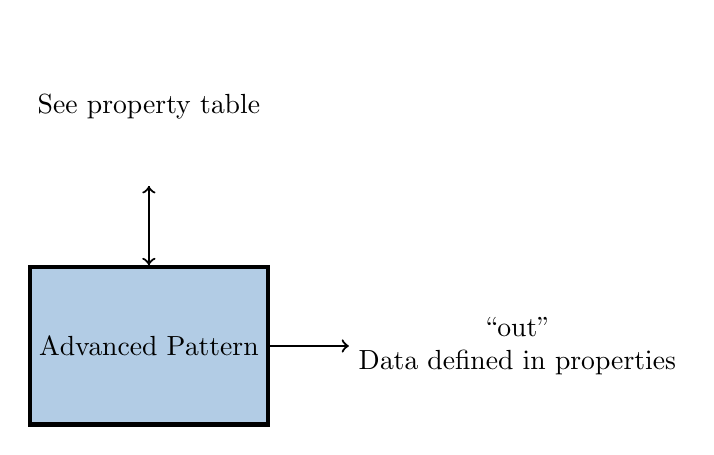
\begin{tikzpicture}[% List of styles applied to all, to override specify on a case-by-case
			every node/.style={
				align=center,  		% use this so that the "\\" for line break works
				minimum size=2cm	% creates space above and below text in rectangle
			},
			every edge/.style={draw,thick}
		]
		\node[rectangle,ultra thick,draw=black,fill=blue](R2){\Comp};
		\node[rectangle,draw=white,fill=white](R4)[right= of R2]{``out'' \\ Data defined in properties};
		\node[rectangle,draw=white,fill=white](R5)[above= of R2]{See property table};
		\path[->]
		(R2)edge []	node [] {} (R4)
		(R2)edge []	node [] {} (R5)
		(R5)edge []	node [] {} (R2)
		;
	\end{tikzpicture}
\end{center}

\section*{Source Dependencies}
\subsection*{\comp.rcc}
\begin{itemize}
	\item $<$assets$>$/components/util\_comps/advanced\_pattern.rcc/advanced\_pattern.cc
\end{itemize}

\begin{landscape}
	\newcounter{fnreadable}
	\section*{Component Spec Properties}
	\begin{scriptsize}
		\begin{minipage}{\textwidth}
			\renewcommand*\footnoterule{} % Remove separator line from footnote
			\renewcommand{\thempfootnote}{\arabic{mpfootnote}} % Use Arabic numbers (or can't reuse)
			\begin{tabular}{|p{3cm}|p{1.5cm}|c|c|c|c|c|p{7cm}|}
				\hline
				\rowcolor{blue}
				Name &
				Type &
				SequenceLength &
				ArrayDimensions &
				Accessibility &
				Valid Range &
				Default &
				Usage \\
				\hline
				\verb+maxPatternLength+ &
				ULong &
				- &
				- &
				Parameter &
				Standard &
				32 &
				Maximum ``\textbf{Pattern}'' sequence length to allow \footnote{Each \textbf{Pattern} entry requires about 2K of RAM.} \\
				\hline
				\verb+Pattern+ &
				Struct &
				\verb+maxPatternLength+ &
				- &
				Initial, Readable\footnote{``Readable'' is deprecated and superfluous here. It will be removed in a future release.}\setcounter{fnreadable}{\thempfootnote} &
				- &
				- &
				Message to send \\
				\hline
				\verb+Pattern.Opcode+ &
				UChar &
				- &
				- &
				'' &
				Standard &
				0 &
				Opcode metadata to send with this message's data \\
				\hline
				\verb+Pattern.Bytes+ &
				UChar &
				2048 &
				- &
				'' &
				Standard &
				0 &
				Data to send \\
				\hline
				\verb+LoopCount+ &
				ULongLong &
				- &
				- &
				Initial, Readable\footnotemark[\thefnreadable] &
				Standard &
				1 &
				How many times to repeat the ``\textbf{Pattern}'' sequence\footnote{0 will continue as long as Worker is running.} \\
				\hline
				\verb+ZLM+ &
				UShort &
				- &
				- &
				Initial, Readable\footnotemark[\thefnreadable] &
				0 \ldots 256 &
				0 &
				Opcode for a \textbf{Z}ero \textbf{L}ength \textbf{M}essage with when finished.\footnote{Default is opcode 0; set to invalid opcode 256 if this feature is \textit{not} desired.} \\
				\hline
				\verb+current+ &
				Struct &
				- &
				- &
				Volatile &
				- &
				- &
				Current statistics for each opcode \\
				\hline
				\verb+current.Total+ &
				Struct &
				- &
				- &
				'' &
				- &
				- &
				Statistics across \textit{all} opcodes \\
				\hline
				\verb+current.Total.bytes+ &
				ULongLong &
				- &
				- &
				'' &
				Standard &
				- &
				Number of bytes received \\
				\hline
				\verb+current.Total.messages+ &
				ULongLong &
				- &
				- &
				'' &
				Standard &
				- &
				Number of messages received \\
				\hline
				\verb+current.Opcode+ &
				Struct &
				- &
				256 &
				'' &
				- &
				- &
				Statistics for \textit{each} opcode \\
				\hline
				\verb+current.Opcode.*+ &
				Various &
				- &
				- &
				'' &
				- &
				Various &
				Various\footnote{Internal structure equivalent to \texttt{current.Total} and not explicitly shown.} \\
				\hline
			\end{tabular}
		\end{minipage}
	\end{scriptsize}
	\section*{Worker Properties}
	There are no implementation-specific properties for this component.

	\section*{Component Ports}
	\begin{scriptsize}
		\begin{tabular}{|M{2cm}|M{1.5cm}|M{4cm}|c|c|M{9cm}|}
			\hline
			\rowcolor{blue}
			Name & Producer & Protocol & Optional & Advanced            & Usage                      \\
			\hline
			out  & true     & -        & -        & numberofopcodes=256 & Data defined in properties \\
			\hline
		\end{tabular}
	\end{scriptsize}

	\section*{Worker Interfaces}
	There are no implementation-specific interfaces for this component.

\end{landscape}
\iffalse
\section*{Performance and Resource Utilization}
\subsubsection*{\comp.rcc}
\begin{scriptsize}
	\begin{tabular}{|c|c|c|}
		\hline
		\rowcolor{blue}
		Processor Type                                & Processor Frequency & Run Function Time \\
		\hline
		linux-c6-x86\_64 Intel(R) Xeon(R) CPU E5-1607 & 3.00 GHz            & TBD               \\
		\hline
		linux-c7-x86\_64 Intel(R) Core(TM) i7-3630QM  & 2.40 GHz            & TBD               \\
		\hline
		linux-x13\_3-arm ARMv7 Processor rev 0 (v7l)  & 666 MHz             & TBD               \\
		\hline
	\end{tabular}
\end{scriptsize}
\fi
\section*{Test and Verification}
The {\comp} worker is tested using five cases. All cases are verified using the md5 hashes of different        properties and or the output file against the expected md5 hashes. A sixth case, {\path{test_05}}, is present but not tested due to sending a ZLM with opcode 1. The {\path{file_write}} component cannot currently stop on ZLM with opcodes other than 0.\\

{\path{case 00}} runs default values and sends a single ZLM with opcode 0. The output file and the contents of the \verb+current+ property are compared to the expected.\\

{\path{case 01}} also runs default values but does not send a ZLM and instead times out after 10 seconds. The \verb+current+ property is compared to the expected.\\

{\path{case 02}} generates the \verb+Pattern+ property {(\path{generate.py} 2)} and sends three bytes every tenth opcode. The \verb+maxPatternLength+ property is explicitly set to be 256. The output file, contents of the \verb+current+ property, and, contents of the \verb+maxPatternLength+ property are compared to the expected.\\

{\path{case 03}} generates the \verb+Pattern+ property {(\path{generate.py} 3)} and sends three bytes every tenth opcode, 50 times. There is no ZLM sent and the test case times out after 10 seconds. The \verb+maxPatternLength+ property is set to 64. For clarity, an {\path{Output_03.out}} file is created to see from where the output hashes are gotten. The output file, contents of the \verb+current+ property, and, contents of the \verb+maxPatternLength+ property are compared to the expected.\\

{\path{case 04}} generates 2048 bytes of data for the \verb+Pattern+ property {(\path{generate.py} 4)} and sends 3 bytes with opcode 0 for 10 seconds. The contents of the \verb+maxPatternLength+ property, and the end cut of the \verb+current+ property are compared to the expected. 
\end{document}
